\documentclass[twoside, 11pt, a4paper]{article}

%%%%%%%%%%%%%%%%%%%%%%%%%%%%%%%%%%%%%%%%%%%%%%%%%%%%%%%%%%%%%%%%%%
% Any additional packages needed should be included after csmr.  %
% Note that csmr.sty includes epsfig, amssymb and graphicx,      %
% and defines many common macros, such as 'proof' and 'example'. %
%%%%%%%%%%%%%%%%%%%%%%%%%%%%%%%%%%%%%%%%%%%%%%%%%%%%%%%%%%%%%%%%%%

\usepackage{csmr}
\usepackage[cp1250]{inputenc}
\usepackage{fancyhdr}

% Definitions of handy macros can go here

%\newcommand{\dataset}{{\cal D}}
%\newcommand{\fracpartial}[2]{\frac{\partial #1}{\partial  #2}}

% Heading arguments are {volume}{nmber}{submitted}{published}{author-full-names}

\csmrheading{8}{2}{2011}

% Short headings should be running head and authors last names

\ShortHeadings{8}{2}{2011}{}{Sorici}

\begin{document}

\title{Argumentational Agent Architecture - Design Principles}

\author{\name Alexandru Sorici\\
       \addr University POLITEHNICA of Bucharest\\
       Faculty of Automatic Control and Computers, Computer Science Department\\
       \email Email: alex.sorici@gmail.com}

\maketitle

\begin{abstract}
The paper presents the design principles used for creating the architecture of an intelligent argumentation agent.
The internal representation of arguments, the communication protocol and message structure (based on the AIF ontology)
will be presented. Finally, a simple use case for the agent and possible future extensions of the model
are presented.
\end{abstract}

\begin{keywords}
Agent architecture, communication protocol, AIF
\end{keywords}

\section{Introduction}

\paragraph*{}
Analyzing communication between entities could not be done throughout history without giving argumentation a great deal of study. 
Argumentation can be defined as the process of putting together a set of statements aimed to strengthen or weaken a claimed expression.
Today the argumentation field has been extended to the computer science and artificial intelligence domain,  especially with areas dealing with multi-agent communication. It has also played a major role in the decision support systems field.
One key challenge is the design of means of communication between intelligent agents. 
Considerable research effort has been expended on the design of artificial languages for agent communications,  such as DARPA's Knowledge Query and Manipulation Language (KQML) [1] and the 
Foundation for Intelligent Physical Agents' (now IEEE FIPA) Agent Communications Language (FIPA ACL) [2].

\paragraph*{}
A variety of systems are now available for users to create and represent arguments such as AML Araucaria [3],  TruthMapping [4], Reason!Able [5], Compendium[6], and others. But, while significant progress has been made in the development of systems
like the latter ones and in understanding the theoretical properties of different argumentation logics and in specifying argumentation dialogues, there remain major barriers to the development and practical deployment of argumentation systems.
These are caused both by a lack of a standard agent architecture and a lack of a shared, agreed notation or "interchange format" for argumentation and arguments. 

\paragraph*{}
The development of a standard agent-based argumentation platform would certainly allow for an easier development of related systems such as Negotiation Systems, Decision support systems etc.
The current paper aims at making an important start towards the removal of the earlier mentioned barriers by presenting the conceptual architecture
of an argumentation agent based on the JADE [7] platform and by presenting an argumentational conversation protocol whose messages rely on the Argumentation Interchange Format (AIF) [8].

\paragraph*{}
The rest of the paper is structured as follows. Section two will introduce related work that explains the structure of the AIF ontology and that describes the usage of dialogue games for modeling agent communication. Section 3 will present the class and protocol diagrams used by the current initial agent architecture. Finally, section 4 will give an example use case and list the future possible extensions of the model.

\section{Related work}
Central to the new agent design are its communication protocol and the representation format of both the internal argument network
and of the exchanged protocol messages. This section introduces work related to the usage of argumentational dialogue games used 
to model agent communication and work related to a standard argument interchange format, the extended AIF ontology.



\section{Agent Architecture and Communication Protocol}

\paragraph*{}Our testing and experimentation framework is based on the above mentioned model of culture dissemination developed by Axelrod. Particularly, we have three main objectives.


\section{Use case and model extensions}


\paragraph*{}In the first experiment, we used the similarity between neigboring individuals as an incentive to make them interact: the interacting neighbor was chosen by means of a roulette process. Each individual had 8 neighbors to choose from. When selecting from all neighbors, apparently opposite to Axelrod's idea that similarity determines even more similarity, the obtained homogeneity regions were not stable. Even though the regions are now perceived as only a set of individuals that share the same feature values, and not necessarily seen as a compact set of cells on the grid, these regions that form over a number of generations are relatively few and their number remains constant. Interestingly enough, this somewhat confirms Axelrod's theory.

\paragraph*{}In the actual baseline simulation (the simple agent), we changed a few minor details, which turned out to have a significant impact on the formation of stable regions. The experiment was run with random interacting agents (not chosen by roulette selection). Moreover the neighborhood was limited to 4 individuals (up, down, left, right). In each generation, a given number of agents were randomly chosen to interact with one of their neighbors. The results were as expected: after a number of generations, the population converged towards a uniform stable region, with very few "islands". In one case we even ended up having the population converge in its entirety. In our simulation, it took the population of 10 x 10 individuals 5000 generations to converge, and populations greater than 15 x 15 individuals took on average more than 15000 iterations to stabilize.

\paragraph*{}For the second type of agent (the balanced agent) we ran the simulation multiple times. Table 1 shows the average convergence time for three different population sizes: 10x10, 15x15, 20x20. As the population increases, only a slight increase in the convergence time can be noticed.



\begin{figure}[htp]
		\centering
		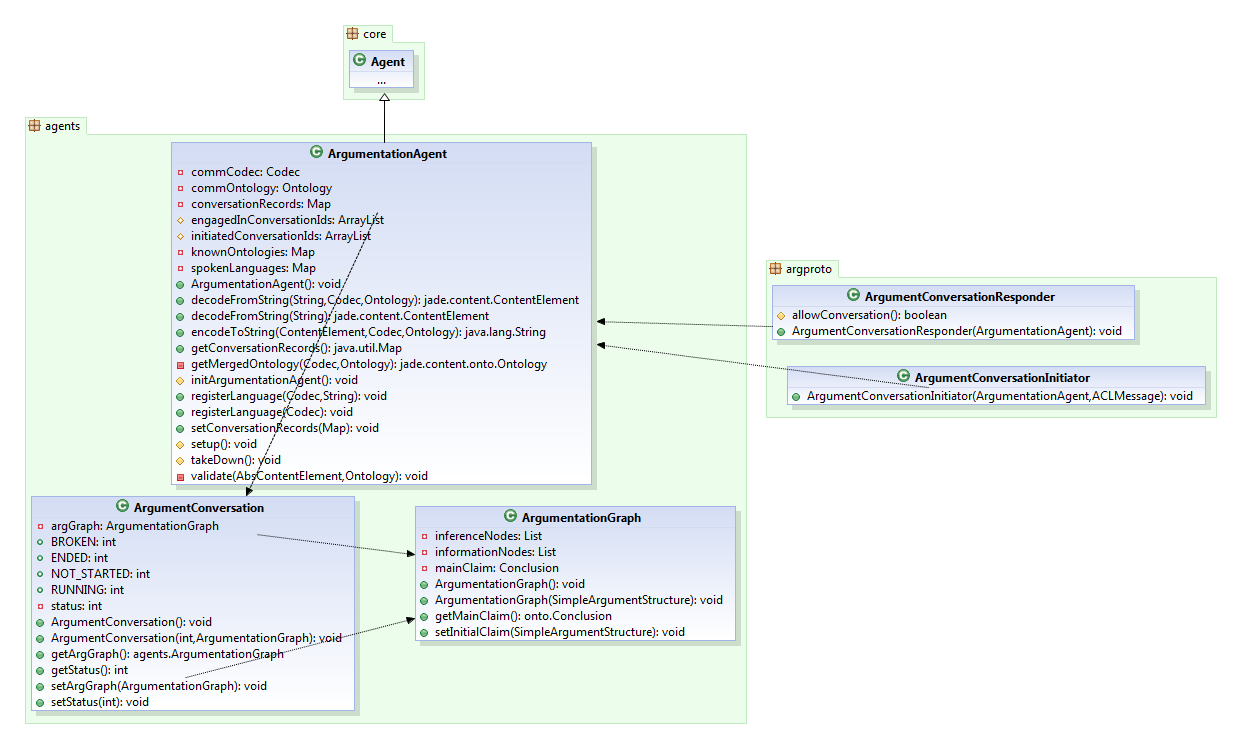
\includegraphics[width=\textwidth]{ArgumentationAgentArchitecture}
		\caption{Class diagram of Argumentation Agent Architecture}
		\label{Fig 1}
\end{figure}

%\newpage
%\pagebreak

\vskip 0.2in
\bibliographystyle{plain}
\bibliography{bibliography}

\end{document}

